\documentclass[12pt]{article}


\usepackage{latexsym}
\usepackage[margin=1in]{geometry}
\usepackage{graphicx}
\usepackage{subfig}
\usepackage{enumerate}
\usepackage{multirow}
\usepackage{booktabs}
%\usepackage{mathptmx}
\usepackage[square]{natbib}
\usepackage{amsmath}
\usepackage{amsfonts}
\usepackage{amssymb}
\usepackage{amsbsy}
\usepackage{amsthm}
\usepackage[pdftex,colorlinks=true,urlcolor=blue,citecolor=black,anchorcolor=black,linkcolor=black]{hyperref}
\usepackage{setspace}

\onehalfspacing

\newtheorem{theorem}{Theorem}
\renewcommand{\thetheorem}{ \arabic{theorem}}
\newtheorem{corollary}[theorem]{Corollary}
\renewcommand{\thecorollary}{\arabic{corollary}}
\newtheorem{definition}{Definition}
\renewcommand{\thedefinition}{\arabic{definition}}
\newtheorem{lemma}{Lemma}
\renewcommand{\thelemma}{ \arabic{lemma}}
\newtheorem{proposition}{Proposition}
\renewcommand{\theproposition}{ \arabic{proposition}}
\newtheorem{remark}{Remark}
\renewcommand{\theremark}{ \arabic{remark}}

% Frequently used general mathematics
\newcommand{\R}{{\mathbb{R}}}
\newcommand{\Rp}{\R^+}
\newcommand{\Z}{{\mathbb{Z}}}
\newcommand{\Zp}{\Z^+}
\newcommand{\Q}{\mathbb{Q}}
\newcommand{\N}{\mathbb{N}}

% Commands for probability
\newcommand{\p}[1]{\mathbb{P} \left\{ #1 \right\}}
\newcommand{\e}[1]{\mathbb{E} \left[ #1 \right]
}
\newcommand{\ee}[2]{\mathbb{E}_{#1} \left[ #2 \right]}
\newcommand{\var}[1]{\mathrm{Var} \left( #1 \right)}
\newcommand{\cov}[1]{\mathrm{Cov} \left( #1 \right)}
\newcommand{\cor}[1]{\mathrm{Corr} \left( #1 \right)}
\newcommand{\varh}[1]{\widehat{\mathrm{Var}} \left( #1 \right)}
\newcommand{\vart}[1]{\widetilde{\mathrm{Var}} \left( #1 \right)}
\newcommand{\vartg}[1]{\widetilde{\mathrm{Var}}_\gamma \left( #1 \right)}
\newcommand{\varhat}{\widehat{\mathrm{Var}}}

% Definitions of variables
\newcommand{\X}{X}
\newcommand{\x}{\mathbf{x}}
\newcommand{\xh}{{\hat{\x}}}
\newcommand{\xs}{\x^*}
\newcommand{\xit}{\boldsymbol{\xi}}
\newcommand{\xiti}{\xit^i}
\newcommand{\zs}{z^*}
\newcommand{\nb}{\left\lfloor\tfrac{n-m}{\gamma}\right\rfloor+1}
\newcommand{\nbl}{\left\lfloor\tfrac{n_l-m_l}{\gamma_l}\right\rfloor+1}
\newcommand{\gammab}{\bar{\gamma}}
\newcommand{\ogb}{\tfrac{1}{\gammab}}
\newcommand{\cogb}{\left\lceil\ogb\right\rceil}

% Definitions for overlapping batches
\newcommand{\gb}{\bar{G}}
\newcommand{\gbb}{\bar{\gb}}
\newcommand{\db}{\bar{D}}
\newcommand{\dbb}{\bar{\db}}

% Used only for review of Meketon.
\newcommand{\y}{\mathbf{y}}
\newcommand{\yb}{\bar{y}}
\newcommand{\ybb}{\bar{\yb}}

\DeclareMathOperator*{\argmin}{argmin}

\newcommand{\Keywords}[1]{\par\noindent 
{\small{\em Keywords\/}: #1}}



%#########################################################
%*
%*  The Document.
%*
\begin{document}

\title{Overlapping Batches for the Assessment of Solution Quality in Stochastic Programs}

\author{David~Love$^{a}$\ \ and G\"{u}zin~Bayraksan$^{b}$\thanks{Corresponding author. Tel.: +1 614-292-1695. Fax:+1 614-292-7852}\\[6pt]
{\small
      $^{a}$ Program in Applied Mathematics, University of Arizona, Tucson, AZ 85721, USA,}\\
{\small \ \ \ \ \ \texttt{dlove@math.arizona.edu}} \\
{\small 
      $^{b}$ Integrated Systems Engineering, The Ohio State University, Columbus, OH 43210, USA,}\\
{\small \ \ \ \  \   \texttt{bayraksan.1@osu.edu}}}
\date{}

\maketitle

\begin{abstract}
\noindent Overlapping Batch Means (OBM) has long been used in simulation as a method of reusing data to generate variance estimators with asymptotically lower variance.
In this paper, we apply the OBM method to stochastic programming by formulating a variant of the multiple replications procedure used for assessing solution quality.
We give conditions under which the resulting optimality gap estimators are strongly consistent and have the same asymptotically lower variance as the classical OBM estimators \citep{Meketon1984,Welch1987}.
Computational experiments for several test problems are presented, examining the small-sample behavior and the computational efficiency of the overlapping batches method in this context.\medskip

\Keywords{Sample average approximation (SAA); Overlapping batch means;   Stochastic programming; Optimality gap estimation}
\end{abstract}

%%%%%%%%%%%%%%%%%%%%%%%%%%%%%%%%%%%%%%%%%%%%%%%%%%%%%%%%%%%%%%%%%%%%%%%%%%%%%%%%
\section{Introduction}
\label{sec:intro}

The Overlapping Batch Means (OBM) method, proposed by \citet{Meketon1984}, is commonly used in simulation to obtain variance estimators having variances that are comparatively lower than their nonoverlapped counterparts. 
In the context of steady-state simulation, OBM is often used to estimate the variance of the sample mean, which is itself an estimator for the mean. 
\cite{SAH90} use overlapping estimators to estimate the variance of estimators for non-means. 
More recently, overlapping estimators based on standardized time series (as opposed to batch means) have been evaluated \citep{Alexopoulos01012007,Alexopoulos2007}; see also \citep{Meterelliyoz_etal_12}.
To the best of our knowledge, OBM has never before been studied in a stochastic optimization context. 
In this paper we show that the same benefits can be obtained from overlapping batches when used in a stochastic optimization setting.
  
A natural setting where batch means are used in stochastic optimization (especially in stochastic programming) is for assessing solution quality. 
This typically involves generating point and interval estimators of the optimality gap of a given candidate solution using Monte Carlo simulation. 
Because optimality gap estimators can be difficult to analyze statistically, a common approach is to use nonovelapping batches of data to generate a number of optimality gap estimators. 
These individual estimators are then used to form point and interval estimators applying the classical nonoverlapping batch means method.
This is referred to as the Multiple Replications Procedure (MRP) and was initially discussed in \citep{Mak1999}.   
In this paper, we formulate an ovelapping batches version of MRP, allowing for partial overlap, and provide conditions under which the resulting gap estimators exhibit reduced variance when compared to their counterparts obtained via nonoverlapping batches.
We also show that the resulting point estimators are strongly consistent and the interval estimators are asymptotically valid. 
We also present computational results to examine small-sample behavior. 
Our experiments indicate that the use of overlapping estimators results in gap estimators achieving lower variance than their nonoverlapping counterparts, along with comparable bias and interval coverage---for both small- and large-sample cases.


We consider a stochastic optimization problem of the form 
\begin{align} \tag{SP} \label{eq:sto_prog} 
	z^* & = \min_{\x \in X} \e{f(\x,\xit)},
\end{align}
where $\x$ is a vector of decision variables, $\xit$ is a vector of random variables, and $X$ is the feasible set, which consists of only deterministic constraints. 
There are no stochastic constraints such as probabilistic or expected-value constraints. 
Further, it is assumed that the distribution of $\xit$ is known and that we can sample from it.
Even though we will impose a more-restrictive moment condition later, we assume that $\e{f(\x,\xit)}$ is well defined and finite for all $\x \in X$ and (\ref{eq:sto_prog}) has a finite optimal solution achieved on $X$.


Unless $f$ has a simple structure or the number of realizations of $\xi$ is small, (\ref{eq:sto_prog}) typically cannot be solved exactly. 
An approximation of (\ref{eq:sto_prog}) can be generated by sampling from the distribution of $\xit$.
While other sampling schemes are possible, let $\xit^1, \xit^2, \dots, \xit^m$ be an independent and identically distributed (i.i.d.) sample from the distribution of $\xit$.
A sampling approximation of (\ref{eq:sto_prog}), often called the sample average approximation, is given by
\begin{align} \tag{SP$_m$} \label{eq:sto_prog_m}
	z_m^* & = \min_{\x \in X} \frac{1}{m} \sum_{i=1}^m f(\x,\xiti).
\end{align}
We denote an optimal solution to (\ref{eq:sto_prog}) as $\xs$ and an optimal solution to (\ref{eq:sto_prog_m}) as $\xs_m$.



We wish to assess the quality of a candidate solution $\xh \in X$. 
Assessing solution quality is important in practice because as (\ref{eq:sto_prog}) typically cannot be solved exactly, one only has an approximate solution $\xh$ without verification of its quality.
Assessing solution quality is also a critical component of stopping criteria in algorithms designed to (approximately) solve (\ref{eq:sto_prog}).
We define the quality of $\xh$ by its optimality gap, $\e{f(\xh,\xit)} - \zs$. 
The lower the optimality gap, the higher the quality of the solution; and a zero optimality gap implies that the solution is optimal. 
Note that the candidate solution $\xh \in X$ may have been found in any way. 
We assume that this solution is given as input to our procedures, and hence fixed, throughout this paper. 


The optimality gap $\e{f(\xh,\xit)} - \zs$ often cannot be calculated exactly. First, for a given candidate solution $\xh \in X$, evaluation of $\e{f(\xh,\xit)}$ typically involves a difficult multidimensional integral. 
Second, we do not know $\zs$. 
In many fields of optimization, the second problem is alleviated by obtaining lower bounds on $\zs$ through relaxations such as integrality, Lagrangian, or semidefinite relations.
As a result, it is common to evaluate an upper bound on the optimality gap. 
This motivates estimating the upper bound on the optimality gap in stochastic programming by using Monte Carlo simulation.
Given a sample size $m$, an upper bound on the optimality gap can be obtained by $$
\e{f(\xh,\xit)} - \zs \leq \e{f(\xh,\xit)} - \e{\zs_m}
$$ 
due to the inequality $\e{\zs_m} \leq \zs$ \citep{Mak1999,norkin_pflug_ruszczynski_98}.
This bound improves as the sample size increases, that is, $\e{\zs_m} \leq \e{\zs_{m+1}} \leq \zs$.  
A straightforward estimate of $\e{f(\xh,\xit)}$ is the sample mean, $\frac{1}{m} \sum_{i=1}^m f(\xh,\xiti)$. 
Instead of $\e{\zs_m}$, we can simply use $\zs_m$.  
The resulting point estimator of the optimality gap is then 
$$
\frac{1}{m} \sum_{i=1}^m f(\xh,\xiti) - \zs_m.
$$ 
Here, we assume the same observations $\xit^1, \dots, \xit^m$ are used in both terms.  

Computing the above optimality gap estimate involves solving an optimization problem (\ref{eq:sto_prog_m}) to obtain a lower bound estimator of $\zs$, $\zs_m$, which complicates the statistical analysis. 
As mentioned above, to enable statistical inference, the MRP of \citet{Mak1999} generates $k$ independent estimators, each using sample size $m$ ($k$ nonoverlapping batches of size $m$) and averages them to obtain a point estimator.  
The sample variance of these estimators is used to form confidence intervals (CIs) for the optimality gap (we further review MRP in \S \ref{ssec:mrp}).  
An advantage of MRP is its applicability to a wide range of problems.  
With i.i.d.\ sampling, $f$ can be linear or nonlinear, $\X$ can include integrality constraints or not.  
It is also easy to implement; thus, MRP has been applied to a wide variety of problems, including finance, supply chain network design, etc.; see, e.g., \citep{bertocchi_etal_99,janjarassuk_linderoth_08,santoso_ahmed_etal_05}.  
Recently, the approach of (nonoverlapping) batching has been used for assessing solution quality of stochastic programs with finitely many expected value \citep{wang_ahmed_08} and stochastic dominance \citep{hu2010sample} constraints.

%When this confidendence interval on the optimality gap is too large, it can be due to three reasons. First, $\xh$ can be far from optimal; second, bias can be large; third, the sampling error can be large. 
%We note that for some problems, bias is a more prominent issue and for others, sampling error is the larger issue. 
%When bias is relatively small, overlapping could help to obtain better variance estimators with simple data reuse, resulting in improved confidence intervals. 


Our aim is to apply the idea of overlapping batches to MRP.  
Overlapping could help to obtain better variance estimators with simple data reuse, resulting in improved CIs.
%Especially for problems where sampling error is dominant, this simple data reuse method could yield better estimators.
We note several differences in this setting compared to the classical setting.  
In simulation output analysis, the point of interest is that of estimating the variance of the sample mean of a covariance stationary process.  
We are interested in estimating the variance of an optimality gap estimator.  
Notice that an optimality gap estimator not only has a sample mean $(\frac{1}{m} \sum_{i=1}^m f(\xh,\xiti))$ but also a minimized sample mean $(\zs_m)$.  
Minimization changes the statistical properties of sample means.  
For instance, the central limit theorem may not hold for a minimized sample mean, even though it holds for each $\x \in \X$.  
Therefore, analysis of the asymptotic benefits of overlapping becomes more complicated.
We overcome this technical difficulty by approximating the optimality gap estimators by their nonoptimized counterparts (see \S \ref{sec:theory}).  
The nonoptimized counterparts are (regular) overlapping batch means estimators (without any optimization present); therefore, they have the desired statistical properties of approximately the same bias and lower variances compared to their nonoverlapping versions. 
We establish convergence of the optimality gap estimators that use overlapping to their nonoptimized counterparts. 
Another difference between our setting and simulation output analysis is that once the data are generated through a simulation, it can be reused without much additional computational effort to obtain the OBM variance estimator.  
In this setting, due to the need to solve a sampling problem (SP$_m$), the computational effort may increase with data reuse.  
This can be alleviated in two ways. 
First, near-optimal variance reduction can be obtained by partially overlapping the batches \citep{Welch1987,Song1992}.  
Partial overlapping results in a smaller number of batches; hence, fewer optimization problems need to be solved.
In this paper, we consider variable amounts of overlap and examine this both theoretically and empirically. 
Second, in many solution methods, warm-starting can be used to quickly solve the sampling approximations with overlapping samples, considerably reducing solution time.




%In this paper, we extend MRP by overlapping the batches similar to the overlapping batch means (OBM) introduced by Meketon and Schmeiser \citep{Meketon1984}. 


%We explore the use of overlapping batches for assessing solution quality in stochastic programs.
%Similar to Welch \citep{Welch1987} and Song and Schmeiser \citep{Song1992}, we consider partial overlap between batches to reduce computational effort in our setting.
%The contributions of this paper are:
%\begin{itemize}
%	\item Formulate the overlapping multiple replications procedure for stochastic programs.
%	\item Give conditions under which the point estimators are strongly consistent (that is, they converge almost surely (a.s.) as opposed in to in probability; referred to simply as consistent from this point on).
%	\item Demonstrate that the classical variance reduction results are achieved for stochastic programs.
%	\item Show the asymptotic validity of the resulting confidence intervals.
%	\item Present computational results on two-stage stochastic linear and integer programs with recourse to examine small sample behavior.  
%		Our experiments indicate that the asymptotic variance reduction is achieved with small sample sizes, while bias and coverage probability are unaffected.
%\end{itemize}

%%%%%%%%%%%%%%%%%%%%%%%%%%%%%%%%%%%%%%%%%%%%%%%%   %    %    %    %    %    %

%\bigskip 

% We present variants of . .  

%\bigskip 

%Batch means have been used in stochastic programming to assess solution quality and we show that. . . 
%\bigskip 


%What happens when overlapping batches are used in a stochastic optimization setting?  Can we obtain the same benefits from overlapping batches as we do in a non-optimized setting?  In this paper, we answer the second question in the affirmative. We provide conditions under which the same benefits can be obtained by overlapping for a class of stochastic optimization problems. A natural setting where batch means is used in stochastic optimization is solution validation. This is referred to as the Multiple Replication Procedure, where each replication is essentially a batch means.  

%\bigskip 
%%%%%%%%%%%%%%%%%%%%%%%%%%%%%%%%%%%%%%%%%%%%%%%%   %    %    %    %    %    %


The rest of the paper is organized as follows.  
In the next section, we review relevant background information.  
We first discuss overlapping batch means in \S \ref{ssec:obm} and then briefly go over MRP in \S \ref{ssec:mrp}.  
In \S \ref{sec:omrp}, we present the Overlapping Multiple Replications Procedure (OMRP) with a parametrized degree of overlap.  
In \S \ref{sec:theory}, we show strong consistency of the OMRP point estimators, asymptotic validity of the OMRP CIs, and that the OMRP variance estimators have lower variances than their nonoverlapping counterparts---the MRP estimators.
In \S \ref{sec:comp}, we test the performance of OMRP on four problems and end in \S \ref{sec:concl} with a summary and conclusions.

%%%%%%%%%%%%%%%%%%%%%%%%%%%%%%%%%%%%%%%%%%%%%%%%%%%%%%%%%%%%%%%%%%%%%%%%%%%%%%%%
\section{Background}
\label{sec:background}

\subsection{Overlapping Batch Means} \label{ssec:obm}
Consider a covariance stationary stochastic process with mean $\mu$ and variance $\sigma^2$.  
The task is to estimate $\mu$ given some realization of the univariate stochastic process $\y = (y^1, y^2, \dots, y^n)$.  
Typically, this involves forming a CI of the form $[L_\alpha(\y), U_\alpha(\y)]$ for a given level of significance $\alpha$ such that $\p{L_\alpha(\y) \leq \mu \leq U_\alpha(\y)} = 1 - \alpha$ or that this probability is approximately $1 - \alpha$ for large enough sample sizes.  
The usual estimator for $\mu$ is the sample mean $\ybb = \frac{1}{n} \sum_{i=1}^n y^i$, which is an unbiased estimator even in the presence of correlated data.  
However, the usual variance estimator $\frac{1}{n-1} \sum_{i=1}^n (y^i - \ybb)^2$ can be inappropriate to use in the presence of correlated data, resulting in inaccurate interval estimators.  
To overcome this difficulty, various variance estimators have been proposed in the simulation literature; see, e.g., \citep{law_07}.  
We briefly review two of these variance estimators: nonoverlapping and overlapping batch means.

Nonoverlapping batch means takes $n$ observations, $y^1, \dots, y^n$ of the stochastic process and splits them into $k$ batches of size $m$, where $k = \frac{n}{m}$ (for simplicity, assume, for now, $n = mk$).  
The sample mean of each batch is then computed as
$
	\yb_j = \frac{1}{m} \sum_{i=1}^{m} y^{m(j-1)+i}, j = 1,2, \dots, k,
$
and the overall sample mean $\ybb = \frac{1}{k} \sum_{j=1}^k \yb_j = \frac{1}{n} \sum_{i=1}^n y^i$ provides a point estimator of $\mu$.  
The variance estimator of the batch means, which is $n/m$ times the sample variance, is calculated as
\begin{equation} \label{eq:var}
	\varhat(\ybb) = \frac{m}{n}\frac{1}{k-1} \sum_{j=1}^k \left( \yb_j - \ybb \right)^2.
\end{equation}
The $(1-\alpha)$-level approximate CI is then formed by $\ybb \pm t_{k-1,\alpha/2} \sqrt{\varhat(\ybb)}$, where $t_{k-1,\alpha/2}$ denotes the $1-\alpha/2$ quantile of the Student's t distribution with $k-1$ degrees of freedom.  
Under appropriate conditions, $n\varhat(\ybb)$ is a consistent estimator of $\sigma^2$.


Overlapping batch means modifies this idea by taking batches given by $\yb_j(m) = \frac{1}{m} \sum_{i=1}^{m}$ $y^{(j-1)+i}$, for $j = 1, \dots, n-m+1$.
As an example, suppose each batch contains $m$ observations and that there are a total of $n=2m$ observations.
In the nonoverlapping case, there are only two batches: the first batch contains observations $y^1, y^2, \dots, y^m$ and the second batch contains observations $y^{m+1}, y^{m+2}, \dots, y^{2m}$.   
In the overlapping batches of \citet{Meketon1984}, the first batch is as before, the second batch now consists of $y^2, y^3, \dots, y^{m+1}$, the third batch contains observations $y^3, y^4, \dots, y^{m+2}$ and so on.  
This is what we call the \emph{maximally-overlapping} batch means method, because $m-1$ observations are common to---and only one observation changes between---adjacent batches.  

The sample variance estimator is updated to
\begin{equation} \label{eq:overlap_variance_def}
	\vart{\ybb} = \frac{1}{(\tfrac{n}{m}-1)(n - m + 1)}\sum_{j=1}^{n-m+1} (\yb_j(m) - \ybb)^2.
\end{equation}
Note that the corresponding overlapping batch means are no longer independent. 
However, by simply reusing the data in this fashion---and seemingly in a contradictory way that induces dependence---one obtains a better variance estimator. 
\citet{Meketon1984} show that: (i) the overlapping variance estimator has nearly the same bias as the standard nonoverlapping variance estimator, and (ii) the overlapping estimator has only two-thirds of the asymptotic variance of the nonoverlapping one.  
That is, 
\begin{equation} \label{eq:asym_var}
	\frac{ \var{\vart{\ybb}} }{ \var{\varhat(\ybb)} } \rightarrow \frac{2}{3}
\end{equation}
in the limit as batch size $m$ and the number of batches $(n/m)$ tend to infinity.  
Note that the degrees of freedom in (\ref{eq:overlap_variance_def}) is slightly different than in \citep{Meketon1984}.  
The degrees of freedom in (\ref{eq:overlap_variance_def}) makes $\vart{\ybb}$ an unbiased estimator for i.i.d.\ data for all finite $m$ and $n$ with the same asymptotic benefits \citep{Song1992}.  
The $(1-\alpha)$-level approximate CI is similarly formed by $\ybb \pm t_{3(k-1)/2,\alpha/2} \sqrt{\vart{\ybb}}$, with an adjustment to the degrees of freedom.

\citet{Welch1987} established the relationship between OBM and spectral estimators and also considered variable amounts of overlap, see also \citep{Song1992}.  
%In our application to assessment of solution quality, we also consider varying the amount of overlap between neighboring batches.  
We defer this discussion on variable overlap to \S \ref{ssec:overlap} and continue with a brief review of MRP.

\subsection{Multiple Replications Procedure} 
\label{ssec:mrp}

%Given a candidate solution $\xh \in \X$ to (\ref{eq:sto_prog}), the task is to estimate its optimality gap $\e{f(\xh,\xit)} - \zs$.  
%Recall that MRP uses the upper bound on the optimality gap, $\e{f(\xh,\xit)} - \e{\zs_m}$ (for a given sample size $m$), to construct a point estimator and a CI using the nonoverlapping batches method described above.  

Taking $n$ observations of the random variables $\xit$ and splitting them into $k$ nonoverlapping batches of size $m$, define 
\begin{align} 
	\gb_j  & = \frac{1}{m} \sum_{i = 1}^{m} f(\xh, \xit^{m(j-1)+i}) - \min_{\x \in X} \frac{1}{m} \sum_{i=1}^{m} f(\x, \xit^{m(j-1)+i}), \ \ \ \ j = 1,2, \dots, k \label{eq:mrp_gap}\\
         & = \frac{1}{m} \sum_{i = 1}^{m} \left[ f(\xh, \xit^{m(j-1)+i}) -  f(\xs_j, \xit^{m(j-1)+i}) \right], \ \ \ \ j = 1,2, \dots, k, \notag
\end{align}
where $\xs_j$ denotes an optimal solution to (\ref{eq:sto_prog_m}) of batch $j$ given on the right-hand side of (\ref{eq:mrp_gap}).    
Since we are assessing the quality of a given solution $\xh \in \X$, we suppress it from the notation $\gb_j$.
The optimality gap estimator $\gb_j$ is similar to $\yb_j$ with individual observations $y^{m(j-1)+i} = f(\xh,\xit^{m(j-1)+i}) - f(\xs_j,\xit^{m(j-1)+i})$, for $i=1,\ldots,m$ and $j=1,\ldots, k$.
Notice that, in this case, $y^i$ not only depends on observation $i$ of batch $j$, $\xit^{m(j-1)+i}$, but all the observations in that batch $\xit^{m(j-1)+1},\xit^{m(j-1)+2},\ldots,\xit^{m(j-1)+m}$ because $\xs_j$ is the optimal solution to (\ref{eq:sto_prog_m}) given in (\ref{eq:mrp_gap}).   
As before, after $k$ estimates are obtained, the overall mean of these estimates $\gbb = \frac{1}{k} \sum_{j=1}^k \gb_j$ provides a point estimator of the optimality gap.  
The sample variance is obtained as in (\ref{eq:var}) by $\varh{\gbb} = \frac{1}{k} \frac{1}{k-1} \sum_{j=1}^k (\gb_j - \gbb)^2$, which results in a one-sided CI $\left[0, \gbb + t_{k-1,\alpha} \sqrt{\varh{\gbb}} \right]$ that has a level of significance, which is approximately $\alpha$.

Notice that the minimization in the second term on the right-hand side of (\ref{eq:mrp_gap}) gives rise to a biased gap estimator (recall the upper bound on the optimality gap).  
Thus, we can expect that the true probability of the optimality gap residing within the CI to be greater than the $1 - \alpha$ suggested by the above calculation.  
This is shown empirically in \citep{Bayraksan2006}, which also investigates additional methods for using a smaller number of replications (e.g., 1 or 2) with an alternative variance estimator to compute a CI.  
See also \citep{bayraksan_morton_09,partani2006jackknife,partani_07} for variations of MRP aimed to reduce bias and variance.



%%%%%%%%%%%%%%%%%%%%%%%%%%%%%%%%%%%%%%%%%%%%%%%%%%%%%%%%%%%%%%%%%%%%%%%%%%%%%%%%
\section{Overlapping Multiple Replications Procedure} 
\label{sec:omrp}

We begin our discussion with variably overlapping batches and then define the estimators of OMRP.

\subsection{Variably Overlapping Batches} 
\label{ssec:overlap}

As before, let $m$ denote the batch size, $n$ the total sample size and $k = \lfloor \tfrac{n}{m} \rfloor$ be the number of nonoverlapping batches.  
In this paper, we use the {\it batch nonoverlap parameter} $1 \leq \gamma \leq m$ to denote how much neighboring batches do {\it not} overlap.  
For instance, $\gamma = m$ corresponds to the classical case of nonoverlapping batches and $\gamma = 1$ corresponds to the maximally overlapping case of \citet{Meketon1984}.  
In general, $\gamma$ can take any integer value between and including $[1,m]$. 
Let $\lfloor \cdot \rfloor$ be the greatest integer that is less than or equal to its argument. 
The sample mean of each batch estimator is calculated similarly, 
$
\yb_j = \frac{1}{m} \sum_{i=1}^m y^{\gamma(j-1) + i},\ \  j = 1, 2, \dots, \nb, 
$
where $\nb$ is the number of batches used given $n$, $m$ and $\gamma$.  
The sample variance estimator given in (\ref{eq:overlap_variance_def}) is changed to
\begin{equation} \label{eq:variance_gamma}
	\vartg{\ybb} = \frac{1}{\left( \tfrac{n}{m} - 1 \right) \left( \nb \right)}  \sum_{j=1}^{\nb} (\yb_j - \ybb)^2.
\end{equation}
Note that with $\gamma=1$, (\ref{eq:variance_gamma}) reduces to (\ref{eq:overlap_variance_def}) and with $\gamma=m$ and $n=mk$, (\ref{eq:variance_gamma}) reduces to (\ref{eq:var}).

The amount of asymptotic variance reduction in this estimator depends on the asymptotic ratio of $\gamma/m$, which we denote by $\gammab$.  
For example, when $\gamma = 1$ (or $\gammab=0$; the maximally overlapping case), the variance is reduced to two-thirds ($66.67\%$) of the original nonoverlapping case, as given in (\ref{eq:asym_var}).  
When 75\% of observations overlap (i.e., when $\gamma = m/4$ or $\gammab = 1/4$), the variance is $33/48$th of the original ($68.75\%$), which is near-optimal.   
When only half of the observations overlap ($\gammab = 1/2$) the variance is 75\% of original.  
Let $\lceil \cdot \rceil$ be the smallest integer that is greater than or equal to its argument. 
In general, from the spectral analysis given in \citep{Welch1987}, the variance is reduced to
\begin{equation} \label{eq:var_reduct_formula}
	\gammab \left( 1 + 2 \sum_{j=1}^{\cogb-1} (1-j\gammab)^2 \right) %= -\gammab\left( 1 - 2\gammab\cogb + \gammab^2\cogb^2 \right) + 2\gammab\cogb\left(1-\gammab\cogb\right) + \frac{2}{3}\gammab^3\cogb^3 + \frac{1}{3}\gammab^3\cogb
\end{equation}
of the nonoverlapping case.  
If $\ogb$ is an integer, (\ref{eq:var_reduct_formula}) simplifies to $\frac{2+\gammab^2}{3}$.


A $(1-\alpha)$-level approximate CI on the mean can be formed using variably overlapping batches by $\ybb \pm t_{d_{\gamma}(k-1),\alpha/2}$ $\sqrt{\vartg{\ybb}}$, where the degrees of freedom increase $d_{\gamma}$ is the multiplicative inverse of (\ref{eq:var_reduct_formula}) \citep{Welch1987}.  
If $\ogb$ is an integer, $d_{\gamma} = \frac{3}{2+\gammab^2}$.  For maximally overlapping batches, the degrees of freedom is $d_{\gamma} = \frac{3}{2}$.
 

\subsection{Definition of Estimators for OMRP}
In order to apply overlapping batches to MRP, we need to keep track of solutions to sampling problems (SP$_m$) for each batch of size $m$.  
Toward this end, let $B(i)$ denote the set of batches $j \in \left\{1, 2, \dots, \nb \right\}$ observation $\xiti$ is used in, $i = 1, 2, \dots, n$.  
See Figure \ref{fig:overlap_nonint} for an example with $n=18$, $m = 6$ and $\gamma = 2$.  
Here, the first batch uses observations $\xit^1, \xit^2, \xit^3, \xit^4, \xit^5, \xit^6$, the second batch uses $\xit^3, \xit^4, \xit^5, \xit^6, \xit^7, \xit^8$, and so on.  
So, $B(1) = \{1\}$, $B(3) = \{1,2\}$, and $B(7)=\{2,3,4\}$.  
As before, we use $\xs_j$ to denote an optimal solution to sampling problem (SP$_m$) formed using the $j$th batch; $\xs_j \in \argmin_{\x \in X} \frac{1}{m} \sum_{i=1}^m f(\x,\xit^{\gamma(j-1) + i})$, $j = 1, 2, \dots, \nb$.

\begin{figure}[htb!]
	\centering
	\begin{tabular}{*{18}{c}}
		$\xit^1$ & $\xit^2$ & $\xit^3$ & $\xit^4$ & $\xit^5$ & $\xit^6$ & $\xit^7$ & $\xit^8$ & $\xit^9$ & $\xit^{10}$ & $\xit^{11}$ & $\xit^{12}$ & $\xit^{13}$ & $\xit^{14}$ & $\xit^{15}$ & $\xit^{16}$ & $\xit^{17}$  & $\xit^{18}$ \\
% 		First Set of Batches
		\multicolumn{6}{l}{[---------------1-----------------]} &
		\multicolumn{6}{l}{[-----------------4------------------]} &
		\multicolumn{6}{l}{[------------------7--------------------]} \\
% 		Third set of Batches
		& & \multicolumn{6}{l}{[---------------2-----------------]} &
		\multicolumn{6}{l}{[------------------5--------------------]} \\
% 		Fifth set of Batches
		& & & & \multicolumn{6}{l}{[---------------3-----------------]} &
		\multicolumn{6}{l}{[------------------6--------------------]} \\
	\end{tabular}
	\caption{Visual representation of overlapping batches with $n = 18$, $m = 6$ and $\gamma = 2$.  
        The brackets show which observations are used in each batch, and the numbers inside each bracket show the batch number $j$.}
	\label{fig:overlap_nonint}
\end{figure}

The results on overlapping batch means occur in the limit as $n, m, k=n/m \rightarrow \infty$ \citep{damerdji1994strong,damerdji1995mean,Meketon1984,Song1992,Welch1987}.  
Let $n_l, m_l$ and $k_l$ be sequences of numbers satisfying these requirements, then the limits will be taken as $l \rightarrow \infty$.  
We assume a batching structure where $m_l = \lfloor n_l ^r \rfloor$ for some $0<r<1$ as is typical in simulation, and $n_l$ tends to infinity as $l \rightarrow \infty$.  
In addition, we may desire that the batch nonoverlap parameter change with $l$, to ensure that $\gamma_l / m_l = \gammab_l$ converges to the constant $\gammab$.  
Now we are ready to define the estimators for OMRP.
\begin{align}
	\gb_{lj} & = \frac{1}{m_l} \sum_{i=1}^{m_l} \left[ f(\xh,\xit^{\gamma_l(j-1)+i}) - f(\xs_j,\xit^{\gamma_l(j-1)+1}) \right],\ \ \ j = 1, 2, \dots, \nbl, \label{eq:gbar} \\
	\gbb_l & = \frac{1}{n_l} \sum_{i=1}^{n_l} \frac{1}{|B(i)|} \sum_{j \in B(i)} \left[ f(\xh,\xiti) - f(\xs_j,\xiti) \right], \label{eq:gbb} \\
	VG_l & = \dfrac{1}{\left( \tfrac{n_l}{m_l} - 1 \right) \left(\nbl\right)} \sum_{j=1}^{\nbl} (\gb_{lj} - \gbb_l)^2. \label{eq:vg}
\end{align}

The optimality gap estimator for each batch $\gb_{lj}$ is defined like (\ref{eq:mrp_gap}) for general values of the nonoverlap parameter $\gamma_l$.  
We just removed the minimization in (\ref{eq:mrp_gap}) and used directly an optimal solution of $\xs_j$ of batch $j$.  
The overall mean, $\gbb_l$, is defined a little differently.  
Here, $\gbb_l$ still uses each observation $i = 1, 2, \dots, n_l$ but also makes use of {\it all} the information collected throughout the batches.  
That is, if observation $\xiti$ is used in $|B(i)|$ number of batches, all the optimal solutions $\xs_j$ corresponding to each batch $j \in B(i)$ are used for the lower bound estimator.  
Then, $VG_l$ is defined in a similar fashion for the variably overlapping batches variance estimator (\ref{eq:variance_gamma}).

%%%%%%%%%%%%%%%%%%%%%%%%%%%%%%%%%%%%%%%%%%%%%%%%%%%%%%%%%%%%%%%%%%%%%%%%%%%%%%%%
\section{Theoretical Results} 
\label{sec:theory}

In this section, we provide conditions under which several asymptotic properties hold. 
First, we show the consistency of the point estimators of optimality gap, $\gbb_l$, and variance, $n_l VG_l$. 
Then, we provide conditions under which the same benefits on variance reduction are observed in the stochastic programming setting by overlapping. 
Finally, we show the asymptotic validity of the OMRP interval estimator. 

\subsection{Assumptions}
\label{subsec:assumptions}

We make the following assumptions:

\begin{description}
	\item[A1] Samples of the random variable $\xit$ are i.i.d.
	\item[A2] $\sup_{\x \in X} \e{f(\x,\xi)^{4}} < \infty$.
	\item[A3] (\ref{eq:sto_prog}) has a unique optimal solution $\xs$ and $\p{\xs_m \neq \xs} \rightarrow 0$ exponentially fast as $m \rightarrow \infty$.  
           That is, there exists constants $M > 0$ and $c > 0$ such that $\log(\p{\xs_m \neq \xs}) \leq -cm$ for all $m > M$.
\end{description}

First, we restrict our attention to i.i.d.\ sampling by A1.
The classical variance-reduction results for overlapping batches show that $\var{n_l VG_l}$ is reduced by overlapping, thus requiring at least finite fourth moments. 
Finally, our proof relies on an exponential rate of convergence of sampled solution to the true solution of the problem.  
Assumption A3 can be satisfied for different classes of problems with unique optimal solutions.  
\citet{shapiro2000rate} establish exponential rates of convergence for a class of (\ref{eq:sto_prog}), which include two-stage stochastic linear programs with recourse when the support of $\xit$ is finite.   
\citet{kleywegt2002sample} show that assumption A3 can be satisfied for discrete stochastic programs (i.e., when $X$ is a finite set) under the condition that the moment generating function of $f(\xs,\xit) - f(\x,\xit)$ for $x \in X \backslash \{\xs\}$ is finite valued on $\R$.  
This class of problems includes stochastic integer programs with recourse.
  We present computational results on both stochastic linear and integer programs with recourse in \S \ref{sec:comp}.

% \begin{description}
% 	\item[A'1] (\ref{eq:sto_prog}) has a unique and sharp optimal solution, i.e., there is a constant $C$ such that $\e{f(\x,\xi)} \geq \e{f(\xs,\xi)} + C\Vert \x - \xs\Vert$ for all $\x \in X$
% 	\item[A'2] (\ref{eq:sto_prog}) is Lipschitz continuous almost surely, i.e., there is a constant $K$ such that $|f(\x_1,\xit) - f(\x_2,\xit)| \leq K \Vert \x_1 - \x_2 \Vert$ for all $\x_1,\x_2 \in X$.

% Some results require an additional assumption:
% \begin{description}
% 	\item[A4] (\ref{eq:sto_prog}) has a unique optimal solution.
% \end{description}



\subsection{Nonoptimimized Counterparts}
\label{subsec:nonO}

The internal optimization in the batches in (\ref{eq:gbar}) makes a straightforward statistical analysis of the behavior of the estimators difficult.  
To overcome this problem, we introduce the following unbiased optimality gap estimators:
\begin{align}
	\db_{lj} & = \frac{1}{m_l} \sum_{i=1}^{m_l} \left[ f(\xh,\xit^{\gamma_l(j-1)+i}) - f(\xs,\xit^{\gamma_l(j-1)+i}) \right],\ \ \ j = 1, 2, \dots, \nbl, \label{eq:dbar} \\
	\dbb_l & = \frac{1}{n_l} \sum_{i=1}^{n_l} \left[ f(\xh,\xiti) - f(\xs,\xiti) \right], \label{eq:dbb} \\
	VD_l & = \frac{1}{\left( \tfrac{n_l}{m_l} - 1 \right) \left(\nbl\right)} \sum_{j=1}^{\nbl} (\db_{lj} - \dbb_l)^2. \label{eq:vd}
\end{align}
These are essentially the same as the variably overlapping batches estimators in \S \ref{ssec:overlap} with $y^i = f(\xh,\xiti) - f(\xs,\xiti)$.  
These are also defined identically to the original estimators (\ref{eq:gbar})--(\ref{eq:vg}) with the exception that $\xs_j$ from (\ref{eq:gbar}) and (\ref{eq:gbb}) is replaced by an optimal solution $\xs$ in (\ref{eq:dbar}) and (\ref{eq:dbb}).  
With $\xh$ and $\xs$ fixed, estimators (\ref{eq:dbar})--(\ref{eq:vd}) have the same statistical properties as variably overlapping batches estimators in \S \ref{ssec:overlap}.  
Note that the optimal solution $\xs$ is not known. 
However, the estimators (\ref{eq:dbar})--(\ref{eq:vd}) are used only to show convergence of (\ref{eq:gbar})--(\ref{eq:vg}); they are not necessary for carrying out the OMRP algorithm.  
Throughout the rest of this section, we assume that the optimality gap estimators (\ref{eq:gbar})--(\ref{eq:vg}) and their nonoptimized counterparts (\ref{eq:dbar})--(\ref{eq:vd}) use identical samples and values of $n_
l$, 
$m_l$, and $\gamma_l$.  \smallskip 


\subsection{Consistency}
\label{subsec:conv} 

We begin with two lemmas that establish exponential rates of convergence of certain intermediate quantities.

\begin{lemma} \label{lem:gbb_prob}
	Under assumptions A1 and A3, $\p{\dbb_l - \gbb_l \neq 0} \rightarrow 0$ exponentially fast as $l \rightarrow \infty$.
\end{lemma}

\begin{proof} When the sampling problems used in the calculation of $\gbb$ all have optimal solutions that solve (SP), i.e., when $\xs_{j} = \xs$, for all $j=1,2,\ldots, \nbl$, then $\gbb_l = \dbb_l$. 
Therefore, probability of the complement of this event provides an upper bound on the probability that $\dbb_l - \gbb_l \neq 0$. 
Let $E^C$ denote the complement of event $E$. 
Using this upper bound and continuing on, we obtain
	\begin{align}
		\p{\dbb_l - \gbb_l \neq 0} & \leq \p{\left( \bigcap_{j=1}^{\nbl} \{\xs_{j} = \xs\} \right)^C} \notag \\
		& = \p{ \bigcup_{j=1}^{\nbl} \{\xs_{j} \neq \xs\}} \notag \\
% 		& \leq \sum_{j=1}^{\nbl} \p{ \xs_j \neq \xs } \notag \\
		& \leq \left( \nbl\right) \p{ \xs_{m_l} \neq \xs }. \notag
	\end{align}
	With a batching structure in which $m_l = \lfloor n_l^{r} \rfloor$ for some $0<r<1$,  $\gamma_l \geq 1$, and by A3, the desired result follows.
\end{proof}

\begin{lemma} \label{lem:gb_gbb_l4}
	Under assumptions A1--A3, both (i) $\e{(\db_{lj} - \gb_{lj})^4} \rightarrow 0$ and (ii) $\e{(\dbb_l - \gbb_l)^4} \rightarrow 0$ exponentially fast as $l \rightarrow \infty$.
\end{lemma}

\begin{proof}
	For brevity, we drop the $lj$ subscripts from $\db_{lj}$ and $\gb_{lj}$ and $l$ from $\gbb_l$ and $\dbb_l$.
	(i) We can decompose the expectation as
	\begin{align*}
		\e{(\db - \gb)^4} & = \e{\left[ \left.(\db - \gb)^4 \right| \db - \gb \neq 0\right]} \p{\db - \gb \neq 0} + 0\\
		& \leq \e{\left[ \left.(\db - \gb)^4 \right| \db - \gb \neq 0 \right]} \p{ \xs_{m_l}  \neq \xs}.
	\end{align*}
	The expectation term on the right-hand side is bounded by assumption A2 for i.i.d.\ samples.  
        Assumption A3 states $\p{\xs_{m_l} \neq \xs} \rightarrow 0$ exponentially fast.  
        Thus $\e{(\db - \gb)^4} \rightarrow 0$ exponentially fast.
(ii) This expectation term can be decomposed in the same manner
	\begin{align*}
		\e{(\dbb - \gbb)^4} & = \e{\left[ \left. (\dbb - \gbb)^4 \right| \dbb - \gbb \neq 0\right]} \p{\dbb - \gbb \neq 0}.
	\end{align*}
	With the expectation term on the right-hand side again bounded by A2, and the probability term converges to zero exponentially fast by Lemma \ref{lem:gbb_prob}.
\end{proof}

We are now ready to show that the resulting point estimators are strongly consistent. 
We use the abbreviation a.s.\ to denote almost sure convergence. 
We also use $\mu_{\xh} := \e{\left[f(\xh,\xit) - f(\xs,\xit)\right]}$ to denote the optimality gap of $\xh$ and $\sigma^2_{\xh} := \var{f(\xh,\xit) - f(\xs,\xit)}$ to denote the associated variance term. 

\begin{theorem} \label{thm:strong_consistency}
	Under assumptions A1--A3, (i) $\gbb_l - \dbb_l \rightarrow 0$, a.s., and (ii) $n_l VG_l - n_l VD_l \rightarrow 0$, a.s.\ as $l \rightarrow \infty$.  
        Therefore, $\gbb_l$ is a consistent estimator of $\mu_{\xh}$, and if $n_l VD_l$ is a consistent estimator of $\sigma^2_{\xh}$, then $n_l VG_l$ is a consistent estimator of $\sigma^2_{\xh}$.
\end{theorem}

\begin{proof}
	(i) By Lemma \ref{lem:gbb_prob}, $\p{\dbb_l - \gbb_l \neq 0}$ $\rightarrow 0$ exponentially fast.  
        Thus $\sum_l \p{\dbb_l - \gbb_l \neq 0} < \infty$.  
        The desired result follows by the Borel-Cantelli Lemma.
%
(ii) This proof is nearly identical to above.  
Note that
	\[
		\p{n_l VD_l -n_l VG_l \neq 0} \leq \p{\left( \bigcap_{j=1}^{\nbl} \{\xs_{j} = \xs\} \right)^C}
	\]
	and by the proof of Lemma \ref{lem:gbb_prob}, $\p{n_l VD_l -n_l VG_l \neq 0} \rightarrow 0$ exponentially fast, and thus $n_l VG_l$ is a consistent estimator of $\sigma^2_{\xh}$, if $n_l VD_l$ is, by the Borel-Cantelli Lemma.
\end{proof}

Part (i) of Theorem \ref{thm:strong_consistency} provides conditions under which the point estimator $\gbb$ of OMRP is a consistent estimator of the optimality gap, by establishing almost sure convergence of $\gbb_l - \dbb_l$ to $0$ as $l \rightarrow \infty$. 
Notice that under assumption A1, $\dbb_l \rightarrow \mu_\xh$, a.s. by the strong law of large numbers; as a result, $\gbb \rightarrow \mu_\xh$, a.s. 
Similarly, part (ii) of Theorem \ref{thm:strong_consistency} establishes almost sure convergence of $n_l VG_l - n_l VD_l$ to $0$ as $l \rightarrow \infty$. 
As a result, if $n_l VD_l$ is a consistent estimator of $\sigma^2_{\xh}$, so is $n_l VG_l$.  
Strong consistency of the variance estimator $n_l VD_l$ has been studied in \citep{damerdji1994strong} for the cases of nonoverlapping and maximally overlapping batches.  
Under the additional moment assumption
\begin{description}
	\item[A2$^\prime$]  $\exists \epsilon > 0$ such that $\sup_{\x \in X} \e{f(\x,\xi)^{4+\epsilon}} < \infty$,
\end{description}
for a sampling scheme of $m_l = \lfloor n_l^r \rfloor$, Corollaries 3.4 and 4.2 of \citep{damerdji1994strong} show that $n_l VD_l$ is consistent if $\tfrac{2}{4+\epsilon} < r < 1$ for nonoverlapping batches and $\tfrac{2}{4+\epsilon} < r < \tfrac{1}{2}$ for maximally overlapping batches. 


\subsection{Variance Reduction}
\label{ssec:var_reduct}

\citet{Meketon1984} show that $\frac{n_l}{m_l}\var{n_l VD_l} \rightarrow \alpha \sigma^4_{\xh}$ where $\alpha = \frac{4}{3}$ for maximally overlapping batches and $\alpha = 2$ for nonoverlapping batches, resulting in the decrease of variance for the maximally overlapping batches estimator.  
\citet{Welch1987} expands this result to variable amounts of overlap, showing that $\alpha$ is twice the value of (\ref{eq:var_reduct_formula}).  
\citet{damerdji1995mean} shows that convergence of $\frac{n_l}{m_l}\var{n_l VD_l}$ to the appropriate $\alpha \sigma^4_{\xh}$---thus the mean-square consistency of $n_l VD_l$---is guaranteed for $\tfrac{1}{2} + \tfrac{1}{4+\epsilon} < r < 1$ for both nonoverlapping and maximally overlapping batches under the batching structure $m_l = \lfloor n_l^r \rfloor$ and $4+\epsilon$ finite moments assumption A2$^\prime$.  
(With A2, the range of $r$ that ensures mean-square consistency can be found by setting $\epsilon=0$.)

To prove the variance reduction results in our setting, we wish to show that 
$$
(\tfrac{n_l}{m_l}) \left( \var{n_l VG_l} - \var{n_l VD_l} \right) \rightarrow 0,
$$
for which it suffices to show $\sqrt{{n_l}/{m_l}} \left( n_l VG_l - n_l VD_l \right) \xrightarrow{L^2} 0$, where $\xrightarrow{L^2}$ denotes mean-square convergence.

%To prove the variance reduction results in our setting, we wish to show that $\frac{\frac{n_l}{m_l} \var{n_lVG_l}}{\frac{n_l}{m_l} \var{n_lVD_l}} \rightarrow 1$.  We do this by showing that $({n_l}/{m_l}) \left( \var{n_l VG_l} - \var{n_l VD_l} \right) \rightarrow 0$, for which it suffices to show $\sqrt{{n_l}/{m_l}} \left( n_l VG_l - n_l VD_l \right) \xrightarrow{L^2} 0$, where $\xrightarrow{L^2}$ denotes mean-square convergence.
%
%\begin{theorem} \label{thm:varvar_conv}
%	Suppose assumptions A1--A3 hold, $\gammab = \frac{\gamma_l}{m_l}$ is constant for all $l$, and the batching structure ensures $nVD_l$ converges in mean-square to $\sigma^2_\xh$.  Then $\dfrac{\frac{n_l}{m_l}\var{nVG_l}}{\frac{n_l}{m_l}\var{nVD_l}} \rightarrow 1$ as $l \rightarrow \infty$.
%\end{theorem}


\begin{theorem} \label{thm:varvar_conv}
	Suppose assumptions A1--A3 hold, $\gammab = \frac{\gamma_l}{m_l}$ is constant for all $l$, and the batching structure ensures  $\frac{n_l}{m_l}\var{n_l VD_l} \rightarrow \alpha \sigma^4_{\xh}$ where $\alpha$ is the twice the value of (\ref{eq:var_reduct_formula}). 
        Then, $\frac{n_l}{m_l}\var{n_l VG_l} \rightarrow \alpha \sigma^4_{\xh}$ as $l \rightarrow \infty$ with the same $\alpha$. 
\end{theorem}

\begin{proof}
	For simplicity of exposition, we drop the subscript $l$ and the $\frac{n_l}{m_l}$ for now and add them in later.  
        Further, we use abbreviations $n_b = \nbl$ to denote the number of batches and $dt = \left(\tfrac{n_l}{m_l} - 1\right) \left(\nbl\right)$ to denote the denominator term in $VG_l$ and $VD_l$. Note that
	\begin{align}
		\e{(nVG - nVD)^2} & = \left( \frac{n}{dt} \right)^2 \e{ \left( \sum_{j=1}^{n_b} \left[ (\gb_j - \gbb)^2 - (\db_j - \dbb)^2 \right] \right)^2 } \notag \\
		& \leq \left( \frac{n}{dt} \right)^2 \e{ n_b \sum_{j=1}^{n_b} \left[ (\gb_j - \gbb)^2 - (\db_j - \dbb)^2 \right]^2 } \label{eq:vvar_conv_pf_1}
	\end{align}
	by the Cauchy-Schwartz inequality, where the second vector in the Cauchy-Schwartz inequality is taken as a vector of ones.  
        By examining the batch structure in Figure \ref{fig:overlap_nonint} and the definition of $\gbb$ in (\ref{eq:gbb}), one can see that the terms of the expectation in (\ref{eq:vvar_conv_pf_1}) are not identically distributed.  
        We will separate these into identically distributed ``center'' batches and ``fringe'' batches.  
        For example, in Figure \ref{fig:overlap_nonint}, only batch 4 is a center batch, while the others are fringe batches.  
        Notice in Figure \ref{fig:overlap_nonint}, we see $\left\lceil \gammab^{-1} \right\rceil = 3$ sets of nonoverlapping batches $\{1,4,7\}$, $\{2,5\}$, and $\{3,6\}$, each of which has two fringe batches.  
        In general, there are $\left\lceil \gammab^{-1} \right\rceil$ sets of nonoverlapping batches, each of which will have two fringe batches, and $n_b - 2\left\lceil \gammab^{-1} \right\rceil$ center batches.
	
	The fringe batches will come in identically distributed pairs.  
        The first and last batch would be identically distributed, as would the second and second-to-last, etc.  
        We know this because we could reverse the order of the i.i.d.\ sample and perform the batching again to get the exact same batch structure.  
        Rewriting to take this into account, letting $A_j = (\gb_j - \gbb)^2 - (\db_j - \dbb)^2$, and continuing from (\ref{eq:vvar_conv_pf_1}),
	\begin{align*}
		& \left( \frac{n}{dt} \right)^2 n_b \e{ \sum_{1}^{n_b} \left[ (\gb_j - \gbb)^2 - (\db_j - \dbb)^2 \right]^2 } \\
		 =  & \left( \frac{n}{dt} \right)^2 n_b \e{\left[ \sum_{j=1}^{\left\lceil \gammab^{-1} \right\rceil} \left[ A_j \right]^2 \
		 + \sum_{j=\left\lceil \gammab^{-1} \right\rceil+1}^{n_b-\left\lceil \gammab^{-1} \right\rceil} \left[ A_j \right]^2 \
		 + \sum_{j=n_b-\left\lceil \gammab^{-1} \right\rceil+1}^{n_b} \left[ A_j \right]^2 \right]\
		} \\
		 = & \left( \frac{n}{dt} \right)^2 n_b \sum_{j=\left\lceil \gammab^{-1} \right\rceil+1}^{n_b-\left\lceil \gammab^{-1} \right\rceil} \e{ \left[ A_j \right]^2 } + \left( \frac{n}{dt} \right)^2 (n_b) 2\sum_{j=1}^{\left\lceil \gammab^{-1} \right\rceil} \e{ \left[ A_j \right]^2 } \\
		 = & \left( \frac{n}{dt} \right)^2 n_b \left(n_b - 2\left\lceil \gammab^{-1} \right\rceil \right) \e{ \left[ A_j \right]^2 }
		+ \left( \frac{n}{dt} \right)^2 (n_b) 2\sum_{j=1}^{\left\lceil \gammab^{-1} \right\rceil} \e{ \left[ A_j \right]^2 }.
	\end{align*}	
	We have $\left\lceil \gammab^{-1} \right\rceil + 1$ expectation terms, each of which has a coefficient that is less than $\left(\frac{n}{dt}\right)^2n_b^2 < (2m)^2$.  
        So each expectation can be bounded by
	\begin{align}
		\left( 2m \right)^2 \e{ \left[ A_j \right]^2 } & = \left( 2m \right)^2 \e{ \left[(\gb_j - \gbb) - (\db_j - \dbb)\right]^2 \left[(\gb_j - \gbb) + (\db_j - \dbb)\right]^2 } \notag \\
		& \leq \left( 2m \right)^2 \sqrt{\e{\left[(\gb_j - \gbb) - (\db_j - \dbb)\right]^4}} \sqrt{\e{\left[(\gb_j - \gbb) + (\db_j - \dbb)\right]^4 }} \label{eq:var_reduct_cauchy2} \\
		& \leq \left( 2m \right)^2 \sqrt{\e{\left[(\gb_j - \gbb) - (\db_j - \dbb)\right]^4}} \sqrt{8 \left(\e{(\gb_j - \gbb)^4} + \e{(\db_j - \dbb)^4} \right)}, \label{eq:var_reduct_holder2}
	\end{align}
	where equation (\ref{eq:var_reduct_cauchy2}) follows from the Cauchy-Schwartz inequality, and equation (\ref{eq:var_reduct_holder2}) follows from H\"{o}lder's inequality.  
        Since we can bound both expectation terms in (\ref{eq:var_reduct_holder2}) by A2, we can demonstrate $\sqrt{\frac{n}{m}}(nVG - nVD) \xrightarrow{L^2} 0$ by focusing on only one of the terms.  
        Focusing on the first expectation term in (\ref{eq:var_reduct_holder2}) and returning the $\tfrac{n}{m}$, by H\"{o}lder's inequality,
	\begin{align*}
		\frac{n}{m} 4m^2 \e{\left[(\gb_j - \gbb) - (\db_j - \dbb)\right]^4}	& \leq 32 \frac{n}{m} m^2\left( \e{(\db_j - \gb_j)^4} + \e{(\dbb - \gbb)^4} \right).
	\end{align*}	
	By Lemma \ref{lem:gb_gbb_l4}, both expectation terms above converge to zero with exponential rates.  
        With a batching structure $m_l = \lfloor n_l^r \rfloor$ for some $0<r<1$, we see that $\frac{n_l}{m_l} \e{(n_l VG_l - n_l VD_l)^2} \rightarrow 0$.
\end{proof} 


Theorem \ref{thm:varvar_conv} shows conditions under which the same asymptotic variance reduction results are achieved for the OMRP optimality gap variance estimator. 
We will empirically examine the variance reduction for small sample sizes in \S \ref{sec:comp}. 
%We end our theoretical properties in the next section by examining the CIs formed using OMRP. 

%%%%%%%%%%%%%%%%%%%%%%%%%%%%%%%%%%%%%%%%%%%%%%%%%%%%%%%%%%%%%%%%%%%%%%%%%%%%%%%%
\subsection{Asymptotic Validity of the Confidence Intervals}

The overlapping variance estimator for stochastic programs displays the same desirable properties as in simulation, but we must still check that it results in a valid CI.  
Let $I^G_l = \gbb_l + t_{d_l,\alpha} \sqrt{VG_l}$ be the width of the one-sided CI generated by OMRP. 
The degrees of freedom $d_l$ is the inverse of (\ref{eq:var_reduct_formula}) using $\frac{\gamma_l}{m_l}$ instead of $\gammab$.

\begin{theorem} \label{thm:conf_int}
	Suppose assumptions A1--A3 hold and the batching structure ensures $n_l VD_l$ converges in probability to $\sigma^2_\xh$.  
        Then, for $\xh \neq \xs$, $\lim_{l\rightarrow\infty} \p{\mu_\xh \leq I^G_l} = 1 - \alpha$.
\end{theorem}

\begin{proof} 
%        With $\xh \neq \xs$, 
			Let $X_l = \frac{\dbb_l - \mu_\xh}{\sigma^2_\xh/\sqrt{n_l}}$, $Y_l = \frac{\gbb_l - \mu_\xh}{\sigma^2_\xh/\sqrt{n_l}}$, and $Z_l = \frac{\sigma^2_\xh}{\sqrt{n_lVD_l}} \frac{\sqrt{n_lVD_l}}{\sqrt{n_lVG_l}}$. 
			Also let $z_{\alpha}$ denote the $1-\alpha$ quantile of the standard normal distribution. 
        It is suffices to show $Y_lZ_l = \frac{\gbb_l - \mu_\xh}{\sqrt{VG_l}} \Rightarrow N(0,1)$, where $\Rightarrow$ denotes convergence in distribution.
			If $\frac{\gbb_l - \mu_\xh}{\sqrt{VG_l}} \Rightarrow N(0,1)$, because $t_{d_l,\alpha} \rightarrow z_{\alpha}$ as $l \rightarrow \infty$, we obtain the desired result by rearranging the terms in $\p{\mu_\xh \leq I^G_l}$ and taking the limit as $l \rightarrow \infty$.
        First, we show that $|X_l - Y_l| \rightarrow 0$, a.s.  Note that $|X_l - Y_l| > 0$ if and only if $|\dbb_l - \gbb_l| > 0$.  
        In the proof of Theorem \ref{thm:strong_consistency} we showed that $\left\{ \dbb_l - \gbb_l \neq 0 \right\}$ happens only finitely many times, so $|X_l - Y_l| \rightarrow 0$, a.s.\ by the Borel-Cantelli Lemma. 
        Next, since $X_l \Rightarrow N(0,1)$  by the central limit theorem and $|X_l - Y_l| \rightarrow 0$ in probability, $Y_l \Rightarrow N(0,1)$.  
        By hypothesis and Theorem \ref{thm:strong_consistency}, $Z_l \rightarrow 1$ in probability.  
        Thus, by Slutsky's theorem, $Y_lZ_l \Rightarrow N(0,1)$.
\end{proof}

The asymptotic validity of the OMRP CI requires $n_l VD_l$ to converge in probability to $\sigma^{2}_{\xh}$. 
This can be achieved either by almost sure or mean-square convergence, which gives a larger range of $r$ in the batching structure.
Also, a hypothesis of Theorem~\ref{thm:conf_int} is that $\xh \neq \xs$.  
For $\xh = \xs$, $\mu_\xh = 0$, and therefore, we have $\lim_{l\rightarrow\infty} \p{\mu_\xh \leq I^G_l} = 1$. 

%%%%%%%%%%%%%%%%%%%%%%%%%%%%%%%%%%%%%%%%%%%%%%%%%%%%%%%%%%%%%%%%%%%%%%%%%%%%%%%
\section{Computational Results}
\label{sec:comp}

In the previous section, we proved asymptotic results regarding the OMRP estimators. 
In this section, we apply OMRP to several test problems and examine small-sample behavior. 
We begin our discussion by introducing the test problems used for numerically evaluating OMRP in \S \ref{ssec:test}, followed by our experimental setup in \S \ref{ssec:expS}. Then, we present and discuss the numerical results in \S \ref{ssec:results}. 

\subsection{Test Problems}
\label{ssec:test}


We empirically tested the effectiveness of OMRP on four test problems.
All test problems are two-stage stochastic programs with recourse and were selected to study the behavior of OMRP under a variety of different situations---we will shortly discuss this below.
The characteristics of these problems are given in Table \ref{tb:test_problems}. 
The first test problem is a newsvendor problem with demand distributed uniformly on $\{0, 0.0001, 0.0002, \dots, 10\}$; we denote it as NVD.
The instance of the newsvendor problem can be found in \citep{Bayraksan2006}, except here we used a discrete uniform demand distribution.
The second is a capacity expansion planning problem, denoted CEP1, with random demand vector $\xit$ of dimension 3, with 216 total realizations \citep{higle1996}.
The third is a stochastic knapsack problem denoted 10D, with 10 stochastic parameters and 10 binary decision variables \citep{kleywegt2002sample}.
The final problem is a stochastic vehicle routing problem, denoted DB1, with 46 stochastic parameters and a total of $4.5 \times 10^{25}$ realizations \citep{donohue1995upper}.


\begin{table}[thb]
\centering
\footnotesize
\begin{tabular}{lcccc}
\hline
& \# of 1st Stage & \# of 2nd Stage & \# of Stochastic & \multirow{2}{*}{\# of Scenarios} \\
Problem & Variables & Variables & Parameters & \\
\cmidrule(r){1-1} \cmidrule(l){2-5}
NVD 	& 1     	& 1     	& 1   	& $10^5 + 1$ \\
CEP1 	& 8     	& 15   	& 3   	& $216$ \\
10D 	& 10     & 1     	& 10   	& $\infty$ \\
DB1 	& 5   	& 102   	& 46   	& $4.5\times 10^{25}$ \\
\hline
\end{tabular}
\caption{Test problem characteristics}
\label{tb:test_problems}
\end{table}



We made several considerations in selecting the test problems.
NVD can be solved very quickly, which allows for solving a large number of independent runs for examining the small-sample behavior of OMRP.
CEP1 is also easy to solve; the optimal solution $\xs$ can be obtained with high probability even for small sample sizes.
This feature shows the behavior of $VG$ when the gap CI width is determined mostly by sampling error, rather than bias.
10D demonstrates the behavior of OMRP when $|X|$ is finite.
Furthermore, 10D has a high condition number \citep{kleywegt2002sample}, making it unlikely that the optimal solution $\xs$ is found when using a sampling solution, thus demonstrating the behavior of OMRP when the bias of the gap is significant.
The optimal solutions of NVD, CEP1, and 10D are known, allowing for explicitly checking and verifying the results.
In contrast, DB1 is a large-scale problem with an unknown optimal solution.
This final test problem allows us to investigate how OMRP works on large-scale problems.


The candidate solutions used for NVD and CEP1 and their characteristics can be found in \citep{Bayraksan2006}.
We used the candidate solution (0, 0, 1, 1, 1, 0, 1, 1, 0, 1) for 10D with $\mu_{\xh} = 158.579$ and the candidate solution (11, 14, 8, 11, 7) for DB1 with an {\it estimated} $\mu_{\xh} = 1.08$. 
Because the optimal solution of DB1 is unknown, a Latin hypercube sample of size 50,000 was used to estimate $\mu_{\xh}$, which was then used below to estimate the coverage probability of the OMRP CIs for this test problem.


\subsection{Experimental Setup}
\label{ssec:expS}


Our experiments were conducted as follows. 
We used a total sample size of $n = 30 m$, with several values of the batch size $m=100, 200, \ldots$. 
Then, at each value of $m$, we formed the OMRP estimators with varying amounts of overlap. 
We also set $\alpha=0.10$, forming 90\% CIs on the optimality gap using the ORMP estimators. 
Results for NVD were compiled over 10,000 independent runs, while the CEP1 and 10D results were taken over 1,000 independent runs, and DB1 results were generated over 500 independent runs.

We solved the sampling approximations of the test problems as follows.
While NVD can be written as a two-stage stochastic linear program with recourse, it can be solved quickly by sorting the demand values. 
We solved it using the quicksort algorithm in C++. 
The problems CEP1 and DB1 are two-stage stochastic linear programs with recourse and were solved with the regularized decomposition algorithm of \citet{ruszczynski1986regularized}, using the accelerated version of the algorithm implemented in C++ \citep{ruszczynski1997accelerating}. 
10D is a stochastic knapsack problem and was solved using dynamic programming.  
In all cases, we used the Mersenne Twister algorithm of \citet{matsumoto_nishimura_98} to generate the random samples, using an implementation in C++ \citep{wagner_twister_09}.




\subsection{Results of Experiments}
\label{ssec:results}

A summary of results from these experiments is depicted in Figures~\ref{fig:varvar1}--\ref{fig:nv}.
Figures~\ref{fig:varvar1} and \ref{fig:varvar2} show the reduction of variance, with each term being normalized with respect to $\var{nVG}$ of the nonoverlapping case (MRP). 
The solid lines in these figures show the theoretical variance reduction from \citep{Welch1987} given by (\ref{eq:var_reduct_formula}). 
Empirical results agree with the theoretical values well, with more variability observed in CEP1, 10D, and DB1. 
These experiments suggest that similar variance reduction can be achieved in stochastic programming by overlapping the batches, even with small sample sizes.
We note that the variance reduction in DB1 can be less than the asymptotic amount. %for the small sample sizes used in these experiments. 
Due its size, DB1 has not yet been solved to optimality, therefore, it may lack a unique optimal solution. 
Even with the relatively small sample sizes compared to the size of this problem, however, overlapping appears to achieve some variance reduction. 


\begin{figure}[htb!]
	\centering
	\subfloat[][NVD]{
	   \label{fig:nv_varvar}
	   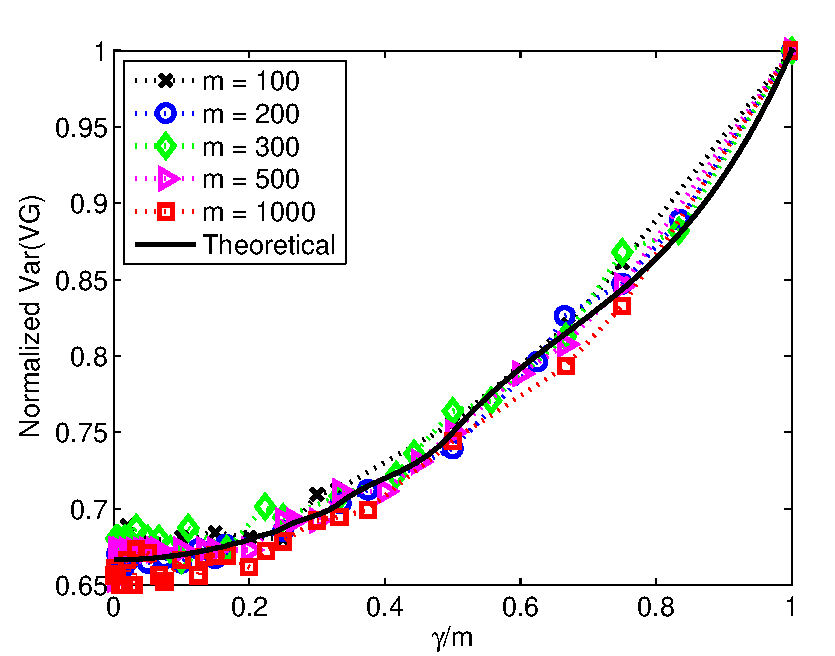
\includegraphics[width=.5\textwidth]{images/nv_varvar_discrete}}
	\subfloat[][CEP1]{
	   \label{fig:cep1_varvar}
	   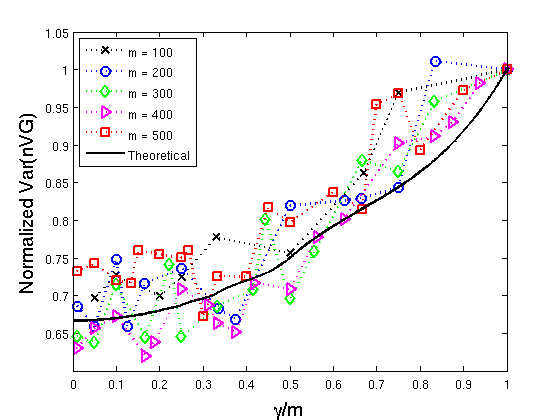
\includegraphics[width=.5\textwidth]{images/cep1_varvar}}
	\caption{
		$\var{n VG}$ relative to the nonoverlapping counterpart across various values of $\gamma/m$ ($\gamma/m=1$ denotes the nonoverlapping batches) for test problem
		(a) NVD, and
		(b) CEP1
	}
\label{fig:varvar1}
\end{figure}

\begin{figure}[htb!]
	\centering
	\subfloat[][10D]{
	   \label{fig:10d_varvar}
	   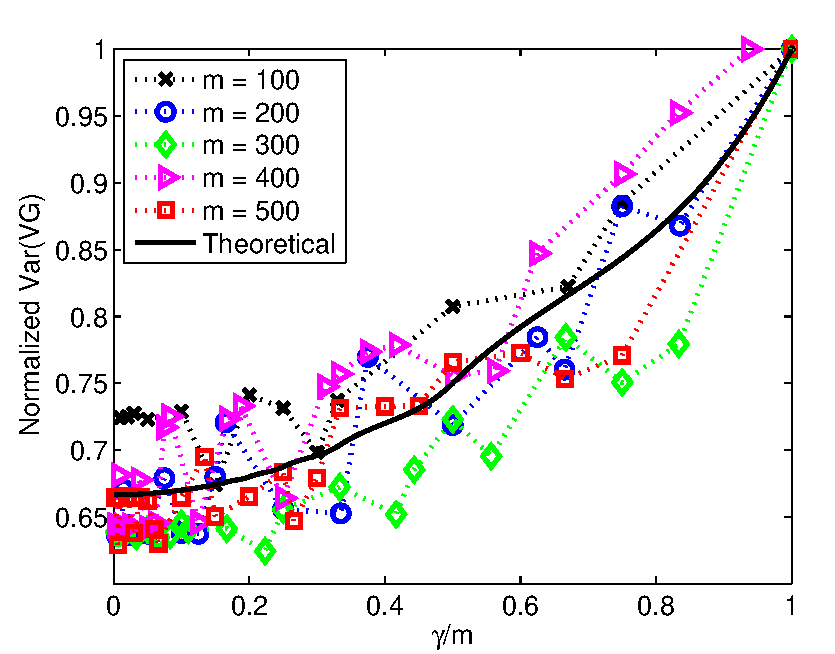
\includegraphics[width=.5\textwidth]{images/10D_varvar}}
	\subfloat[][DB1]{
	   \label{fig:db1_varvar}
	   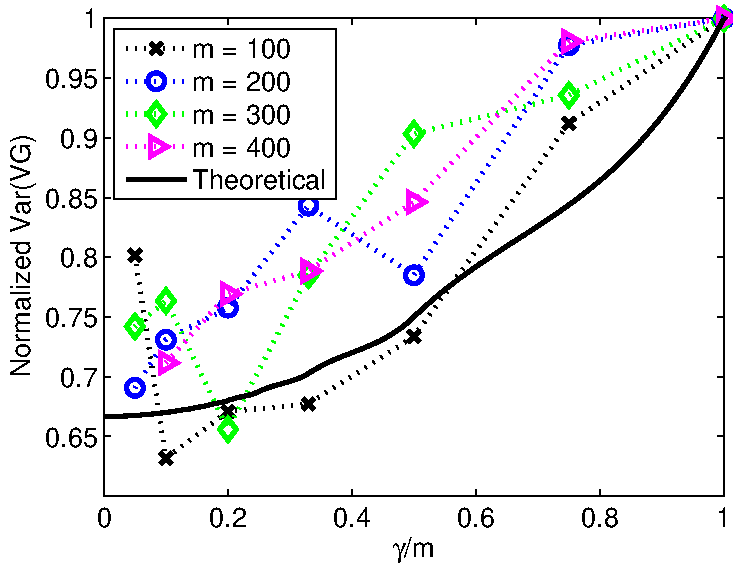
\includegraphics[width=.5\textwidth]{images/db1_varvar}}
		\caption{
		$\var{n VG}$ relative to the nonoverlapping counterpart across various values of $\gamma/m$ ($\gamma/m=1$ denotes the nonoverlapping batches) for test problem
		(a) 10D, and
		(b) DB1
		}
\label{fig:varvar2}
\end{figure}


\begin{figure}[htb!]
	\centering
	\subfloat[][Expected Variance]{
	   \label{fig:nv_avgvar}
	   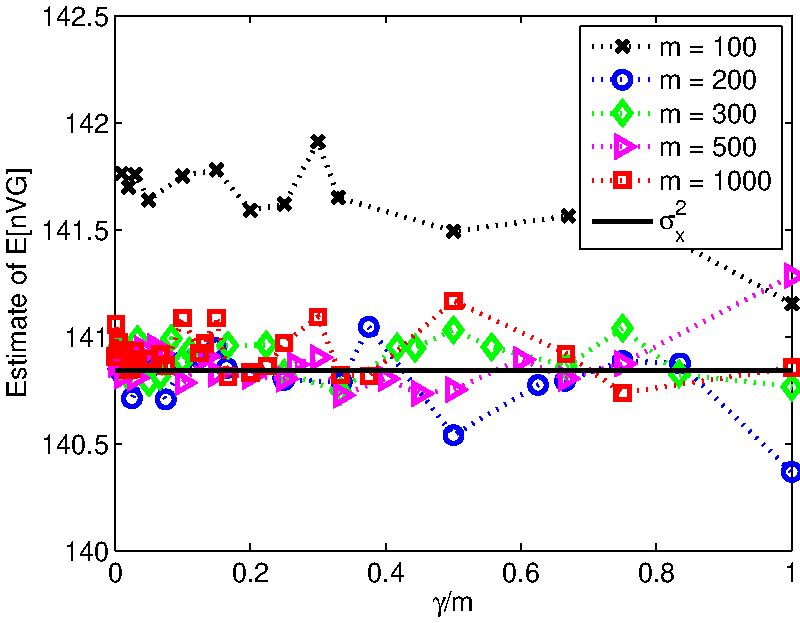
\includegraphics[width=.5\textwidth]{images/nv_avgvar_discrete}}
	\subfloat[][Coverage Probability]{
	   \label{fig:nv_cover}
	   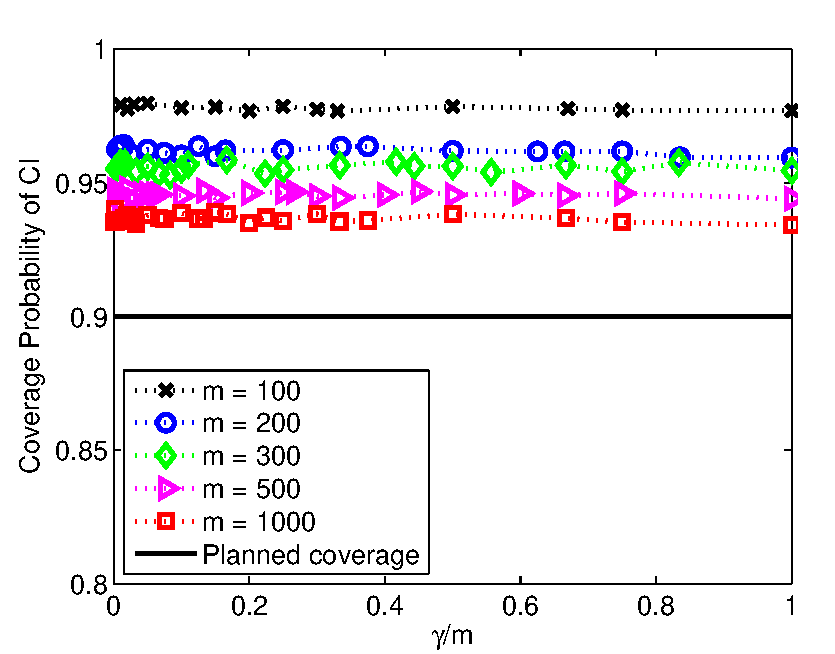
\includegraphics[width=.5\textwidth]{images/nv_cover_discrete}}
	\caption{ 
		Estimates of
		(a) $\e{nVG}$, and 
		(c) coverage probability of the CIs for various values of $\gamma/m$ ($\gamma/m=1$ denotes the nonoverlapping batches)
		 for NVD
	}
\label{fig:nv}
\end{figure}


Figure~\ref{fig:nv}(a) shows estimates of $\e{nVG}$ in the newsvendor problem for changing batch size and amount of overlap. 
We can see that the expectation of the variance estimator is not changed with increasing overlap. 
Although the estimate of $\e{nVG}$ looks large for $m=100$, the error from $\sigma^2_\xh$ is never more than 1\%.  
Estimates for $\e{nVG}$ showed a similar pattern for CEP1, 10D, and DB1.  
Those graphs are omitted for brevity.

Finally, Figure~\ref{fig:nv}(b) shows the coverage probability of CIs generated by OMRP for several values of $m$ across varying values of $\gamma/m$ for the newsvendor problem.  
The results of the classical overlapping batches estimators show that coverage probability does not change with the amount of overlap, which we can  empirically see in this figure for OMRP for NVD.
We observed the same for CEP1, 10D, and DB1.  
The coverage probabilities from applying the (nonoverlapping) MRP algorithm to these problems presented in \citep{Bayraksan2006} agree with our results: for the newsvendor problem, coverage probability drops as $m$ increases and the coverage probability of CEP1 (not shown) remains fairly constant around the desired value of $90\%$. 
Coverage probability for 10D (not shown) and {\it estimated} coverage probability for DB1 (also not shown) were very high, more than $0.99$.  
The bias from solving (\ref{eq:sto_prog_m}) for these problems seems to be much more significant than the variance.

\subsection{Computational Efficiency}
\label{ssec:compeff}

xxx Add new graphs here \bigskip 

xxx Write new text, etc. \bigskip 

xxx Revise the recommendations on gammabar \bigskip 

Because variance reduction drops quickly as $\gammab$ drops below $1$, we recommend using an intermediate value of $\gammab$, such as $1/3$ or $1/4$, to gain the majority of the variance reduction, while reducing the number of optimization problems to be solved. 
Warm-starting the algorithm to solve the sampling problems, when such as scheme is available, can significantly reduce the computation times.

%%%%%%%%%%%%%%%%%%%%%%%%%%%%%%%%%%%%%%%%%%%%%%%%%%%%%%%%%%%%%%%%%%%%%%%%%%%%%%%
\section{Conclusions}
\label{sec:concl}

We have extended previous work from simulation output analysis to assessing solution quality in stochastic programming by means of variably overlapping batches \citep{Meketon1984,Song1992,Welch1987} for Monte Carlo simulation-based estimators of optimality gaps in stochastic programs \citep{Mak1999}. 
We have provided conditions under which the resulting point estimator of the optimality gap and its associated sample variance are consistent, the same variance reduction can be achieved, and asymptotically valid CIs can be formed. 
Empirical results with small sample sizes indicate that the asymptotic reductions in variance of the variance estimator show a similar decrease in OMRP, while bias and coverage probability remain unaffected. 

%%%%%%%%%%%%%%%%%%%%%%%%%%%%%%%%%%%%%%%%%%%%%%%%%%%%%%%%%%%%%%%%%%%%%%%%%%%%%%%
\section*{Acknowledgments}
The authors thank Andrzej Ruszczy{\'{n}}ski and Artur {\'{S}}wietanowski for
access to their regularized decomposition code, which was used to solve CEP1 and DB1. 
The authors are also grateful to the associate editor and two anonymous referees for valuable suggestions that significantly improved both the content and the presentation of the paper. 
%This research has been supported in part by the National Science Foundation under Grant(s)  EFRI-0835930 and CMMI-1345626 ??? 
An earlier version of this paper appeared in \citep{love2011overlapping}.

%%%%%%%%%%%%%%%%%%%%%%%%%%%%%%%%%%%%%%%%%%%%%%%%%%%%%%%%%%%%%%%%%%%%%%%%%%%%%%%
\bibliographystyle{abbrvnat}
\bibliography{omrp}
%%%%%%%%%%%%%%%%%%%%%%%%%%%%%%%%%%%%%%%%%%%%%%%%%%%%%%%%%%%%%%%%%%%%%%%%%%%%%%%

\end{document}
